% Difference table of f(x)=x^3+x+1 for x=0..5; left edge = Newton coefficients. Generated by a short script.
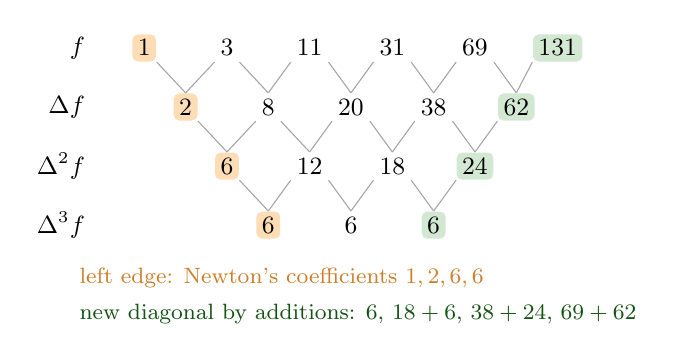
\begin{tikzpicture}[x=1.05cm,y=0.75cm,every node/.style={font=\small}]
\node[anchor=east] at (-0.6,0) {$f$};
\node[fill=BurntOrange!25,rounded corners=2pt,inner sep=2pt] (n00) at (0.0,0) {$1$};
\node[,inner sep=2pt] (n01) at (1.0,0) {$3$};
\node[,inner sep=2pt] (n02) at (2.0,0) {$11$};
\node[,inner sep=2pt] (n03) at (3.0,0) {$31$};
\node[,inner sep=2pt] (n04) at (4.0,0) {$69$};
\node[fill=ForestGreen!20,rounded corners=2pt,inner sep=2pt] (n05) at (5.0,0) {$131$};
\node[anchor=east] at (-0.6,-1) {$\Delta f$};
\node[fill=BurntOrange!25,rounded corners=2pt,inner sep=2pt] (n10) at (0.5,-1) {$2$};
\node[,inner sep=2pt] (n11) at (1.5,-1) {$8$};
\node[,inner sep=2pt] (n12) at (2.5,-1) {$20$};
\node[,inner sep=2pt] (n13) at (3.5,-1) {$38$};
\node[fill=ForestGreen!20,rounded corners=2pt,inner sep=2pt] (n14) at (4.5,-1) {$62$};
\node[anchor=east] at (-0.6,-2) {$\Delta^2f$};
\node[fill=BurntOrange!25,rounded corners=2pt,inner sep=2pt] (n20) at (1.0,-2) {$6$};
\node[,inner sep=2pt] (n21) at (2.0,-2) {$12$};
\node[,inner sep=2pt] (n22) at (3.0,-2) {$18$};
\node[fill=ForestGreen!20,rounded corners=2pt,inner sep=2pt] (n23) at (4.0,-2) {$24$};
\node[anchor=east] at (-0.6,-3) {$\Delta^3f$};
\node[fill=BurntOrange!25,rounded corners=2pt,inner sep=2pt] (n30) at (1.5,-3) {$6$};
\node[,inner sep=2pt] (n31) at (2.5,-3) {$6$};
\node[fill=ForestGreen!20,rounded corners=2pt,inner sep=2pt] (n32) at (3.5,-3) {$6$};
\draw[gray!70] (n00.south east)--(n10.north);\draw[gray!70] (n01.south west)--(n10.north);
\draw[gray!70] (n01.south east)--(n11.north);\draw[gray!70] (n02.south west)--(n11.north);
\draw[gray!70] (n02.south east)--(n12.north);\draw[gray!70] (n03.south west)--(n12.north);
\draw[gray!70] (n03.south east)--(n13.north);\draw[gray!70] (n04.south west)--(n13.north);
\draw[gray!70] (n04.south east)--(n14.north);\draw[gray!70] (n05.south west)--(n14.north);
\draw[gray!70] (n10.south east)--(n20.north);\draw[gray!70] (n11.south west)--(n20.north);
\draw[gray!70] (n11.south east)--(n21.north);\draw[gray!70] (n12.south west)--(n21.north);
\draw[gray!70] (n12.south east)--(n22.north);\draw[gray!70] (n13.south west)--(n22.north);
\draw[gray!70] (n13.south east)--(n23.north);\draw[gray!70] (n14.south west)--(n23.north);
\draw[gray!70] (n20.south east)--(n30.north);\draw[gray!70] (n21.south west)--(n30.north);
\draw[gray!70] (n21.south east)--(n31.north);\draw[gray!70] (n22.south west)--(n31.north);
\draw[gray!70] (n22.south east)--(n32.north);\draw[gray!70] (n23.south west)--(n32.north);
\node[anchor=west,font=\footnotesize,text=BurntOrange!80!black] at (-0.9,-3.9) {left edge: Newton's coefficients $1,2,6,6$};
\node[anchor=west,font=\footnotesize,text=ForestGreen!60!black] at (-0.9,-4.5) {new diagonal by additions: $6$, $18+6$, $38+24$, $69+62$};
\end{tikzpicture}
